\chapter{Hardware}

I det følgende afsnit beskrives systemets hardware vha. SysML diagrammer. 
Indledningsvis bruges block definition diagrammer til at identificere og beskrive systemets blokke. Senere i afsnittet åbnes udvalgte blokke og de interne og eksterne forbindelser vises med internal block diagrammer. 
I det følgende vil det block definition diagrammer blive kaldt bdd'er, og internal block diagrammer benævnes ibd'er. 

\section{Block definition diagram}
I det overordnede bdd nedenfor vises de blokke systemet består af, samt hvilke parts blokkene har. Helt overordnet set består systemet af blokkene: \textit{Webserver} og \textit{Drone}. 

\begin{figure}[H]
\centering
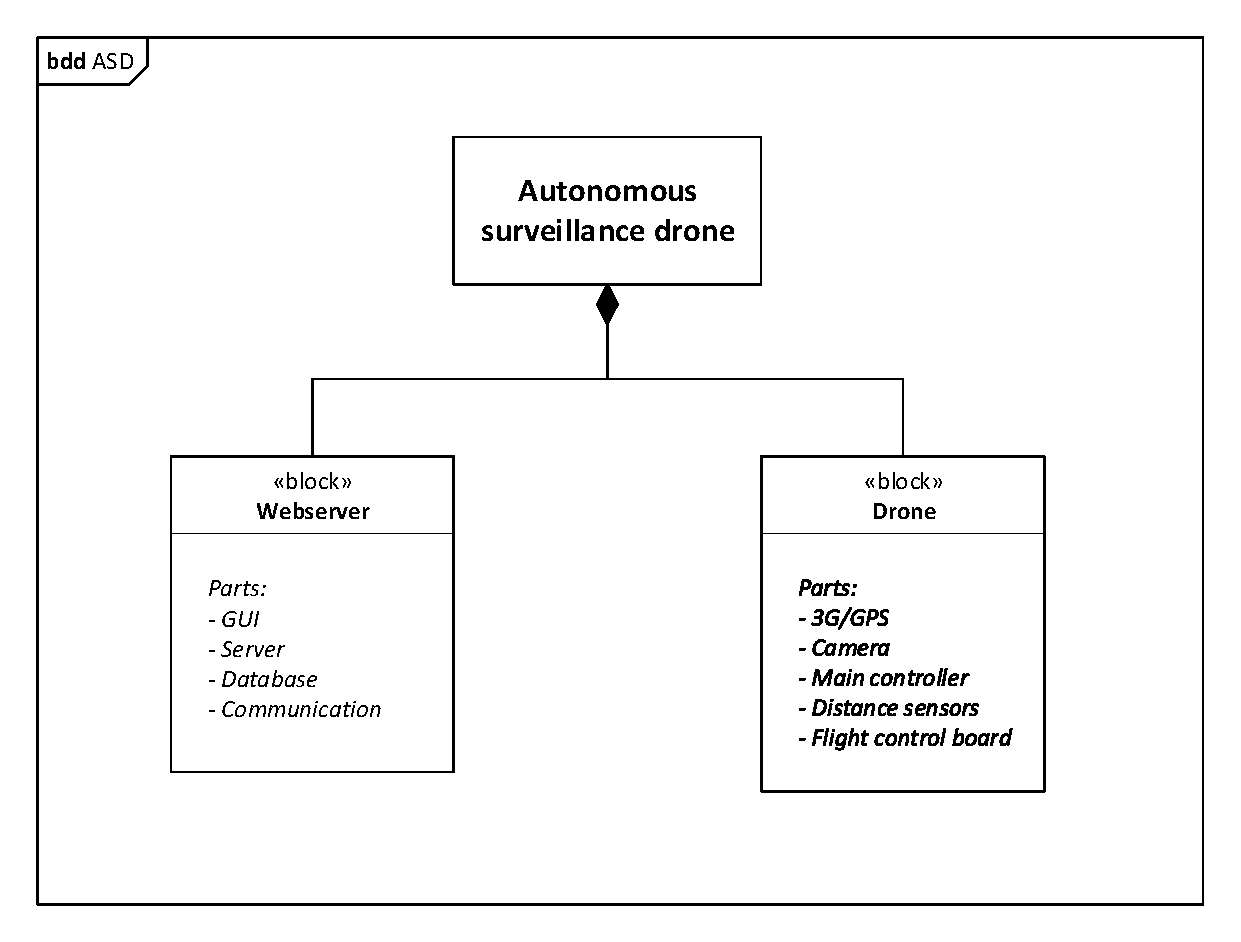
\includegraphics[width=1\textwidth]{Billeder/BDD/bdd_overordnet.pdf}
\vspace{-0.5cm}
\caption{Bdd - overordnet}
\label{fig:bdd_overordnet}
\end{figure}

\newpage
\subsection{Udvidet - Block definition diagram}
Da drone blokken er kompliceret og indeholder mange parts kræves en yderlige beskrivelse. På figur \ref{fig:bdd_drone} vises et bdd, der går mere i dybden med drone blokken. På figuren åbnes drone blokken og det vises hvilke blokke dronen er bygget af. 

\begin{figure}[H]
\centering
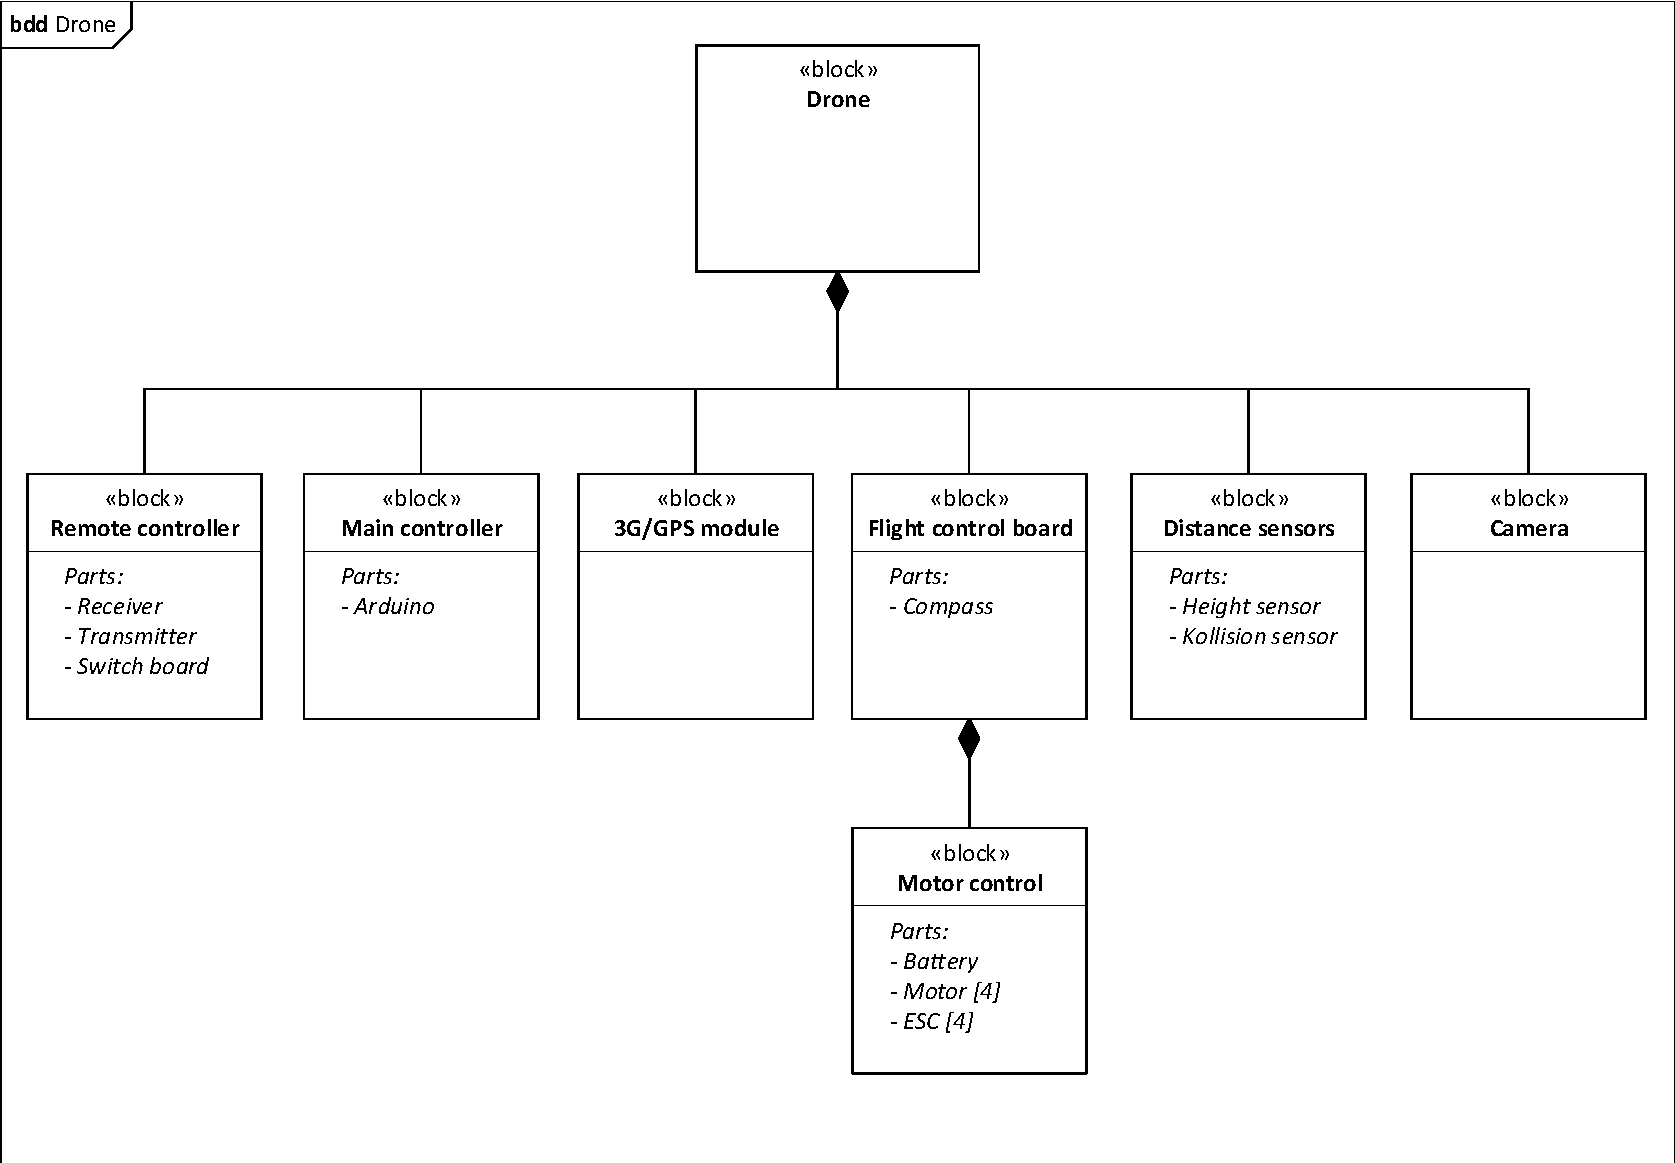
\includegraphics[width=1.\textwidth]{Billeder/BDD/bdd_drone.pdf}
\vspace{-0.5cm}
\caption{Bdd - drone}
\label{fig:bdd_drone}
\end{figure}

\vspace{0.5cm}

Webserveren beskrives ikke nærmere i dette afsnit, da den ikke indeholder så mange parts og fordi webserverens parts har en anden og mere løs kobling end dronens.

\newpage

\subsection{Blokbeskrivelse}

\textbf{Main controller}\\
Main controlleren fungerer som dronens hjerne. Ud fra kommunikation med webserver og input fra de forskellige sensorer styrer main controlleren dronens motorer. Skal dronen fx. flyve højere udsendes styrings signaler, som sørger for motorerne øger deres rotationshastighed. Under autonom flyvning bruges PWM signaler udsendt fra main controller til styre dronen. 

\textbf{Remote controller}\\
Denne blok består af receiver, transmitter og switch board. Blokken gør det muligt at switche mellem autonom og manuel styring. Afhængig af hvordan transmitteren (fjernbetjening) er indstillet benyttes henholdsvis manuel eller autonom flyvning.

\textbf{Flight control board}\\
Flight control boardet indholder software til styring, derunder PID regulering. Boardet har indbygget kompas, gyroskop, accelerometer og barometer, som alle bruges under flyvning. Flight control boardets vigtigste opgave er at viderebringe control signaler fra main controller til ESC'er som åbner/lukker for forsyning til dronens motorer. 

\textbf{3G/GPS module}\\
3G/GPS blokken har to funktioner i systemet. For det første er 3G/GPS blokken ansvarlig for opdatering af dronens GPS position. Desuden fungerer blokken som kommunikationslag mellem webserver og main controller. Al information der udvekles mellem webserver og drone går gennem 3G/GPS modulet.

\textbf{Distance sensorer}\\
Afstands sensorerne bruges både til måling af flyvehøjde og til anti kollision. Sensorerne aktiveres af main controlleren, når højdemåling eller tjek af forhindring foretages. Sensorerne bruger 40 kHz signaler til at måle distancen til jorden eller eventuelle forhindringer.

\textbf{Camera}\\
Når dronen er i rette position modtager kameraet besked og tager et billede. Billedet tages og sendes videre i systemet til godkendelse. Der tages et nyt billede hvis billedet ikke godkendes.

\textbf{Motor control}\\
Denne blok består af ESC, batteri og motorer. Blokken styres med PWM signaler, som udsendes fra flight control boardet.

\textbf{Webserver}\\
Denne blok indeholder server, webapplikation, database og communikation. 
Ved interaktion med webapplikation er det muligt for bruger at tilgå server. Sammenspil mellem webapplikation og server gør det muligt for bruger at lave en ny flyveopsætning eller undersøge en tidligere flyvning. Server kommunikerer med dronen og gemmer løbende vigtig information i databasen.
